% Options for packages loaded elsewhere
\PassOptionsToPackage{unicode}{hyperref}
\PassOptionsToPackage{hyphens}{url}
\PassOptionsToPackage{dvipsnames,svgnames,x11names}{xcolor}
%
\documentclass[
  12pt,
]{article}

\usepackage{amsmath,amssymb}
\usepackage{iftex}
\ifPDFTeX
  \usepackage[T1]{fontenc}
  \usepackage[utf8]{inputenc}
  \usepackage{textcomp} % provide euro and other symbols
\else % if luatex or xetex
  \usepackage{unicode-math}
  \defaultfontfeatures{Scale=MatchLowercase}
  \defaultfontfeatures[\rmfamily]{Ligatures=TeX,Scale=1}
\fi
\usepackage{lmodern}
\ifPDFTeX\else  
    % xetex/luatex font selection
\fi
% Use upquote if available, for straight quotes in verbatim environments
\IfFileExists{upquote.sty}{\usepackage{upquote}}{}
\IfFileExists{microtype.sty}{% use microtype if available
  \usepackage[]{microtype}
  \UseMicrotypeSet[protrusion]{basicmath} % disable protrusion for tt fonts
}{}
\makeatletter
\@ifundefined{KOMAClassName}{% if non-KOMA class
  \IfFileExists{parskip.sty}{%
    \usepackage{parskip}
  }{% else
    \setlength{\parindent}{0pt}
    \setlength{\parskip}{6pt plus 2pt minus 1pt}}
}{% if KOMA class
  \KOMAoptions{parskip=half}}
\makeatother
\usepackage{xcolor}
\ifLuaTeX
  \usepackage{luacolor}
  \usepackage[soul]{lua-ul}
\else
  \usepackage{soul}
  
\fi
\setlength{\emergencystretch}{3em} % prevent overfull lines
\setcounter{secnumdepth}{-\maxdimen} % remove section numbering
% Make \paragraph and \subparagraph free-standing
\makeatletter
\ifx\paragraph\undefined\else
  \let\oldparagraph\paragraph
  \renewcommand{\paragraph}{
    \@ifstar
      \xxxParagraphStar
      \xxxParagraphNoStar
  }
  \newcommand{\xxxParagraphStar}[1]{\oldparagraph*{#1}\mbox{}}
  \newcommand{\xxxParagraphNoStar}[1]{\oldparagraph{#1}\mbox{}}
\fi
\ifx\subparagraph\undefined\else
  \let\oldsubparagraph\subparagraph
  \renewcommand{\subparagraph}{
    \@ifstar
      \xxxSubParagraphStar
      \xxxSubParagraphNoStar
  }
  \newcommand{\xxxSubParagraphStar}[1]{\oldsubparagraph*{#1}\mbox{}}
  \newcommand{\xxxSubParagraphNoStar}[1]{\oldsubparagraph{#1}\mbox{}}
\fi
\makeatother

\usepackage{color}
\usepackage{fancyvrb}
\newcommand{\VerbBar}{|}
\newcommand{\VERB}{\Verb[commandchars=\\\{\}]}
\DefineVerbatimEnvironment{Highlighting}{Verbatim}{commandchars=\\\{\}}
% Add ',fontsize=\small' for more characters per line
\usepackage{framed}
\definecolor{shadecolor}{RGB}{241,243,245}
\newenvironment{Shaded}{\begin{snugshade}}{\end{snugshade}}
\newcommand{\AlertTok}[1]{\textcolor[rgb]{0.68,0.00,0.00}{#1}}
\newcommand{\AnnotationTok}[1]{\textcolor[rgb]{0.37,0.37,0.37}{#1}}
\newcommand{\AttributeTok}[1]{\textcolor[rgb]{0.40,0.45,0.13}{#1}}
\newcommand{\BaseNTok}[1]{\textcolor[rgb]{0.68,0.00,0.00}{#1}}
\newcommand{\BuiltInTok}[1]{\textcolor[rgb]{0.00,0.23,0.31}{#1}}
\newcommand{\CharTok}[1]{\textcolor[rgb]{0.13,0.47,0.30}{#1}}
\newcommand{\CommentTok}[1]{\textcolor[rgb]{0.37,0.37,0.37}{#1}}
\newcommand{\CommentVarTok}[1]{\textcolor[rgb]{0.37,0.37,0.37}{\textit{#1}}}
\newcommand{\ConstantTok}[1]{\textcolor[rgb]{0.56,0.35,0.01}{#1}}
\newcommand{\ControlFlowTok}[1]{\textcolor[rgb]{0.00,0.23,0.31}{\textbf{#1}}}
\newcommand{\DataTypeTok}[1]{\textcolor[rgb]{0.68,0.00,0.00}{#1}}
\newcommand{\DecValTok}[1]{\textcolor[rgb]{0.68,0.00,0.00}{#1}}
\newcommand{\DocumentationTok}[1]{\textcolor[rgb]{0.37,0.37,0.37}{\textit{#1}}}
\newcommand{\ErrorTok}[1]{\textcolor[rgb]{0.68,0.00,0.00}{#1}}
\newcommand{\ExtensionTok}[1]{\textcolor[rgb]{0.00,0.23,0.31}{#1}}
\newcommand{\FloatTok}[1]{\textcolor[rgb]{0.68,0.00,0.00}{#1}}
\newcommand{\FunctionTok}[1]{\textcolor[rgb]{0.28,0.35,0.67}{#1}}
\newcommand{\ImportTok}[1]{\textcolor[rgb]{0.00,0.46,0.62}{#1}}
\newcommand{\InformationTok}[1]{\textcolor[rgb]{0.37,0.37,0.37}{#1}}
\newcommand{\KeywordTok}[1]{\textcolor[rgb]{0.00,0.23,0.31}{\textbf{#1}}}
\newcommand{\NormalTok}[1]{\textcolor[rgb]{0.00,0.23,0.31}{#1}}
\newcommand{\OperatorTok}[1]{\textcolor[rgb]{0.37,0.37,0.37}{#1}}
\newcommand{\OtherTok}[1]{\textcolor[rgb]{0.00,0.23,0.31}{#1}}
\newcommand{\PreprocessorTok}[1]{\textcolor[rgb]{0.68,0.00,0.00}{#1}}
\newcommand{\RegionMarkerTok}[1]{\textcolor[rgb]{0.00,0.23,0.31}{#1}}
\newcommand{\SpecialCharTok}[1]{\textcolor[rgb]{0.37,0.37,0.37}{#1}}
\newcommand{\SpecialStringTok}[1]{\textcolor[rgb]{0.13,0.47,0.30}{#1}}
\newcommand{\StringTok}[1]{\textcolor[rgb]{0.13,0.47,0.30}{#1}}
\newcommand{\VariableTok}[1]{\textcolor[rgb]{0.07,0.07,0.07}{#1}}
\newcommand{\VerbatimStringTok}[1]{\textcolor[rgb]{0.13,0.47,0.30}{#1}}
\newcommand{\WarningTok}[1]{\textcolor[rgb]{0.37,0.37,0.37}{\textit{#1}}}

\providecommand{\tightlist}{%
  \setlength{\itemsep}{0pt}\setlength{\parskip}{0pt}}\usepackage{longtable,booktabs,array}
\usepackage{calc} % for calculating minipage widths
% Correct order of tables after \paragraph or \subparagraph
\usepackage{etoolbox}
\makeatletter
\patchcmd\longtable{\par}{\if@noskipsec\mbox{}\fi\par}{}{}
\makeatother
% Allow footnotes in longtable head/foot
\IfFileExists{footnotehyper.sty}{\usepackage{footnotehyper}}{\usepackage{footnote}}
\makesavenoteenv{longtable}
\usepackage{graphicx}
\makeatletter
\def\maxwidth{\ifdim\Gin@nat@width>\linewidth\linewidth\else\Gin@nat@width\fi}
\def\maxheight{\ifdim\Gin@nat@height>\textheight\textheight\else\Gin@nat@height\fi}
\makeatother
% Scale images if necessary, so that they will not overflow the page
% margins by default, and it is still possible to overwrite the defaults
% using explicit options in \includegraphics[width, height, ...]{}
\setkeys{Gin}{width=\maxwidth,height=\maxheight,keepaspectratio}
% Set default figure placement to htbp
\makeatletter
\def\fps@figure{htbp}
\makeatother

\usepackage{booktabs}
\usepackage{longtable}
\usepackage{array}
\usepackage{multirow}
\usepackage{wrapfig}
\usepackage{float}
\usepackage{colortbl}
\usepackage{pdflscape}
\usepackage{tabu}
\usepackage{threeparttable}
\usepackage{threeparttablex}
\usepackage[normalem]{ulem}
\usepackage{makecell}
\usepackage{xcolor}
\usepackage{setspace}
\setstretch{1.0}
\usepackage{geometry}
\geometry{margin=0.6in}
\usepackage{parskip}
\setlength{\parskip}{0.3em}
\setlength{\parindent}{0.1em}
\usepackage{listings}
\lstset{breaklines=true}
\usepackage{graphicx}
\usepackage{longtable}
\usepackage{caption}
\captionsetup{width=\textwidth}
\makeatletter
\@ifpackageloaded{caption}{}{\usepackage{caption}}
\AtBeginDocument{%
\ifdefined\contentsname
  \renewcommand*\contentsname{Table of contents}
\else
  \newcommand\contentsname{Table of contents}
\fi
\ifdefined\listfigurename
  \renewcommand*\listfigurename{List of Figures}
\else
  \newcommand\listfigurename{List of Figures}
\fi
\ifdefined\listtablename
  \renewcommand*\listtablename{List of Tables}
\else
  \newcommand\listtablename{List of Tables}
\fi
\ifdefined\figurename
  \renewcommand*\figurename{Figure}
\else
  \newcommand\figurename{Figure}
\fi
\ifdefined\tablename
  \renewcommand*\tablename{Table}
\else
  \newcommand\tablename{Table}
\fi
}
\@ifpackageloaded{float}{}{\usepackage{float}}
\floatstyle{ruled}
\@ifundefined{c@chapter}{\newfloat{codelisting}{h}{lop}}{\newfloat{codelisting}{h}{lop}[chapter]}
\floatname{codelisting}{Listing}
\newcommand*\listoflistings{\listof{codelisting}{List of Listings}}
\makeatother
\makeatletter
\makeatother
\makeatletter
\@ifpackageloaded{caption}{}{\usepackage{caption}}
\@ifpackageloaded{subcaption}{}{\usepackage{subcaption}}
\makeatother

\ifLuaTeX
  \usepackage{selnolig}  % disable illegal ligatures
\fi
\usepackage{bookmark}

\IfFileExists{xurl.sty}{\usepackage{xurl}}{} % add URL line breaks if available
\urlstyle{same} % disable monospaced font for URLs
\hypersetup{
  pdftitle={STATS 506 : HW-5},
  pdfauthor={Vasudha Rohatgi},
  colorlinks=true,
  linkcolor={blue},
  filecolor={Maroon},
  citecolor={Blue},
  urlcolor={Blue},
  pdfcreator={LaTeX via pandoc}}


\title{STATS 506 : HW-5}
\author{Vasudha Rohatgi}
\date{}

\begin{document}
\maketitle


\paragraph{\texorpdfstring{Code hosted at
\url{https://github.com/Vasu2499/HW-5}}{Code hosted at https://github.com/Vasu2499/HW-5}}\label{code-hosted-at-httpsgithub.comvasu2499hw-5}

\subsection{Problem - 1}\label{problem---1}

\textbf{\emph{OOP Programming}}

\subsubsection{\texorpdfstring{1 - \texttt{Constructor} and
\texttt{Validator} (with rationality
check)~}{1 - Constructor and Validator (with rationality check)~}}\label{constructor-and-validator-with-rationality-check}

\begin{Shaded}
\begin{Highlighting}[]
\FunctionTok{library}\NormalTok{(methods)}

\CommentTok{\# Rational S4 class}
\FunctionTok{setClass}\NormalTok{(}
  \StringTok{"Rational"}\NormalTok{,}
  \AttributeTok{slots =} \FunctionTok{list}\NormalTok{(}
    \AttributeTok{numerator =} \StringTok{"numeric"}\NormalTok{,}
    \AttributeTok{denominator =} \StringTok{"numeric"}
\NormalTok{  ),}
  \AttributeTok{validity =} \ControlFlowTok{function}\NormalTok{(object) \{}
    \ControlFlowTok{if}\NormalTok{ (object}\SpecialCharTok{@}\NormalTok{denominator }\SpecialCharTok{==} \DecValTok{0}\NormalTok{) \{}
      \FunctionTok{return}\NormalTok{(}\StringTok{"Denominator cannot be zero."}\NormalTok{)}
\NormalTok{    \}}
    \ConstantTok{TRUE}
\NormalTok{  \}}
\NormalTok{)}

\CommentTok{\# Constructor function}
\NormalTok{rational }\OtherTok{\textless{}{-}} \ControlFlowTok{function}\NormalTok{(numerator, denominator) \{}
  \FunctionTok{new}\NormalTok{(}\StringTok{"Rational"}\NormalTok{, }\AttributeTok{numerator =}\NormalTok{ numerator, }\AttributeTok{denominator =}\NormalTok{ denominator)}
\NormalTok{\}}
\end{Highlighting}
\end{Shaded}

\subsubsection{\texorpdfstring{3 - \texttt{Show}
Method}{3 - Show Method}}\label{show-method}

\begin{Shaded}
\begin{Highlighting}[]
\FunctionTok{setMethod}\NormalTok{(}
  \StringTok{"show"}\NormalTok{,}
  \StringTok{"Rational"}\NormalTok{,}
  \ControlFlowTok{function}\NormalTok{(object) \{}
    \FunctionTok{cat}\NormalTok{(}\FunctionTok{paste0}\NormalTok{(object}\SpecialCharTok{@}\NormalTok{numerator, }\StringTok{"/"}\NormalTok{, object}\SpecialCharTok{@}\NormalTok{denominator, }\StringTok{"}\SpecialCharTok{\textbackslash{}n}\StringTok{"}\NormalTok{))}
\NormalTok{  \}}
\NormalTok{)}
\end{Highlighting}
\end{Shaded}

\subsubsection{\texorpdfstring{4 - \texttt{Simplify}
Method}{4 - Simplify Method}}\label{simplify-method}

\begin{Shaded}
\begin{Highlighting}[]
\FunctionTok{library}\NormalTok{(Rcpp)}
\end{Highlighting}
\end{Shaded}

\begin{verbatim}
Warning: package 'Rcpp' was built under R version 4.4.2
\end{verbatim}

\begin{Shaded}
\begin{Highlighting}[]
\CommentTok{\# Define GCD and LCM functions}
\NormalTok{Rcpp}\SpecialCharTok{::}\FunctionTok{cppFunction}\NormalTok{(}\StringTok{"}
\StringTok{int gcd(int a, int b) \{}
\StringTok{  while (b != 0) \{}
\StringTok{    int temp = b;}
\StringTok{    b = a \% b;}
\StringTok{    a = temp;}
\StringTok{  \}}
\StringTok{  return a;}
\StringTok{\}}
\StringTok{"}\NormalTok{)}

\CommentTok{\# Simplify method}
\FunctionTok{setGeneric}\NormalTok{(}\StringTok{"simplify"}\NormalTok{, }\ControlFlowTok{function}\NormalTok{(object) }\FunctionTok{standardGeneric}\NormalTok{(}\StringTok{"simplify"}\NormalTok{))}
\end{Highlighting}
\end{Shaded}

\begin{verbatim}
[1] "simplify"
\end{verbatim}

\begin{Shaded}
\begin{Highlighting}[]
\FunctionTok{setMethod}\NormalTok{(}
  \StringTok{"simplify"}\NormalTok{,}
  \StringTok{"Rational"}\NormalTok{,}
  \ControlFlowTok{function}\NormalTok{(object) \{}
\NormalTok{    g }\OtherTok{\textless{}{-}} \FunctionTok{gcd}\NormalTok{(object}\SpecialCharTok{@}\NormalTok{numerator, object}\SpecialCharTok{@}\NormalTok{denominator)}
\NormalTok{    object}\SpecialCharTok{@}\NormalTok{numerator }\OtherTok{\textless{}{-}}\NormalTok{ object}\SpecialCharTok{@}\NormalTok{numerator }\SpecialCharTok{/}\NormalTok{ g}
\NormalTok{    object}\SpecialCharTok{@}\NormalTok{denominator }\OtherTok{\textless{}{-}}\NormalTok{ object}\SpecialCharTok{@}\NormalTok{denominator }\SpecialCharTok{/}\NormalTok{ g}
\NormalTok{    object}
\NormalTok{  \}}
\NormalTok{)}
\end{Highlighting}
\end{Shaded}

\subsubsection{\texorpdfstring{5 - \texttt{Quotient}
Method}{5 - Quotient Method}}\label{quotient-method}

\begin{Shaded}
\begin{Highlighting}[]
\CommentTok{\# Quotient method}
\FunctionTok{setGeneric}\NormalTok{(}\StringTok{"quotient"}\NormalTok{, }\ControlFlowTok{function}\NormalTok{(object, }\AttributeTok{digits =} \DecValTok{7}\NormalTok{) }\FunctionTok{standardGeneric}\NormalTok{(}\StringTok{"quotient"}\NormalTok{))}
\end{Highlighting}
\end{Shaded}

\begin{verbatim}
[1] "quotient"
\end{verbatim}

\begin{Shaded}
\begin{Highlighting}[]
\FunctionTok{setMethod}\NormalTok{(}
  \StringTok{"quotient"}\NormalTok{,}
  \StringTok{"Rational"}\NormalTok{,}
  \ControlFlowTok{function}\NormalTok{(object, }\AttributeTok{digits =} \DecValTok{7}\NormalTok{) \{}
    \ControlFlowTok{if}\NormalTok{ (}\SpecialCharTok{!}\FunctionTok{is.numeric}\NormalTok{(digits) }\SpecialCharTok{||}\NormalTok{ digits }\SpecialCharTok{\textless{}=} \DecValTok{0}\NormalTok{) \{}
      \FunctionTok{stop}\NormalTok{(}\StringTok{"Digits must be a positive numeric value."}\NormalTok{)}
\NormalTok{    \}}
\NormalTok{    res }\OtherTok{\textless{}{-}}\NormalTok{ object}\SpecialCharTok{@}\NormalTok{numerator }\SpecialCharTok{/}\NormalTok{ object}\SpecialCharTok{@}\NormalTok{denominator}
    \FunctionTok{cat}\NormalTok{(}\FunctionTok{format}\NormalTok{(res, }\AttributeTok{digits =}\NormalTok{ digits), }\StringTok{"}\SpecialCharTok{\textbackslash{}n}\StringTok{"}\NormalTok{)}
\NormalTok{    res}
\NormalTok{  \}}
\NormalTok{)}

\CommentTok{\# Arithmetic methods}
\FunctionTok{setMethod}\NormalTok{(}\StringTok{"+"}\NormalTok{, }\FunctionTok{signature}\NormalTok{(}\AttributeTok{e1 =} \StringTok{"Rational"}\NormalTok{, }\AttributeTok{e2 =} \StringTok{"Rational"}\NormalTok{), }\ControlFlowTok{function}\NormalTok{(e1, e2) \{}
\NormalTok{  numerator }\OtherTok{\textless{}{-}}\NormalTok{ e1}\SpecialCharTok{@}\NormalTok{numerator }\SpecialCharTok{*}\NormalTok{ e2}\SpecialCharTok{@}\NormalTok{denominator }\SpecialCharTok{+}\NormalTok{ e2}\SpecialCharTok{@}\NormalTok{numerator }\SpecialCharTok{*}\NormalTok{ e1}\SpecialCharTok{@}\NormalTok{denominator}
\NormalTok{  denominator }\OtherTok{\textless{}{-}}\NormalTok{ e1}\SpecialCharTok{@}\NormalTok{denominator }\SpecialCharTok{*}\NormalTok{ e2}\SpecialCharTok{@}\NormalTok{denominator}
  \FunctionTok{simplify}\NormalTok{(}\FunctionTok{rational}\NormalTok{(numerator, denominator))}
\NormalTok{\})}

\FunctionTok{setMethod}\NormalTok{(}\StringTok{"{-}"}\NormalTok{, }\FunctionTok{signature}\NormalTok{(}\AttributeTok{e1 =} \StringTok{"Rational"}\NormalTok{, }\AttributeTok{e2 =} \StringTok{"Rational"}\NormalTok{), }\ControlFlowTok{function}\NormalTok{(e1, e2) \{}
\NormalTok{  numerator }\OtherTok{\textless{}{-}}\NormalTok{ e1}\SpecialCharTok{@}\NormalTok{numerator }\SpecialCharTok{*}\NormalTok{ e2}\SpecialCharTok{@}\NormalTok{denominator }\SpecialCharTok{{-}}\NormalTok{ e2}\SpecialCharTok{@}\NormalTok{numerator }\SpecialCharTok{*}\NormalTok{ e1}\SpecialCharTok{@}\NormalTok{denominator}
\NormalTok{  denominator }\OtherTok{\textless{}{-}}\NormalTok{ e1}\SpecialCharTok{@}\NormalTok{denominator }\SpecialCharTok{*}\NormalTok{ e2}\SpecialCharTok{@}\NormalTok{denominator}
  \FunctionTok{simplify}\NormalTok{(}\FunctionTok{rational}\NormalTok{(numerator, denominator))}
\NormalTok{\})}

\FunctionTok{setMethod}\NormalTok{(}\StringTok{"*"}\NormalTok{, }\FunctionTok{signature}\NormalTok{(}\AttributeTok{e1 =} \StringTok{"Rational"}\NormalTok{, }\AttributeTok{e2 =} \StringTok{"Rational"}\NormalTok{), }\ControlFlowTok{function}\NormalTok{(e1, e2) \{}
\NormalTok{  numerator }\OtherTok{\textless{}{-}}\NormalTok{ e1}\SpecialCharTok{@}\NormalTok{numerator }\SpecialCharTok{*}\NormalTok{ e2}\SpecialCharTok{@}\NormalTok{numerator}
\NormalTok{  denominator }\OtherTok{\textless{}{-}}\NormalTok{ e1}\SpecialCharTok{@}\NormalTok{denominator }\SpecialCharTok{*}\NormalTok{ e2}\SpecialCharTok{@}\NormalTok{denominator}
  \FunctionTok{simplify}\NormalTok{(}\FunctionTok{rational}\NormalTok{(numerator, denominator))}
\NormalTok{\})}

\FunctionTok{setMethod}\NormalTok{(}\StringTok{"/"}\NormalTok{, }\FunctionTok{signature}\NormalTok{(}\AttributeTok{e1 =} \StringTok{"Rational"}\NormalTok{, }\AttributeTok{e2 =} \StringTok{"Rational"}\NormalTok{), }\ControlFlowTok{function}\NormalTok{(e1, e2) \{}
\NormalTok{  numerator }\OtherTok{\textless{}{-}}\NormalTok{ e1}\SpecialCharTok{@}\NormalTok{numerator }\SpecialCharTok{*}\NormalTok{ e2}\SpecialCharTok{@}\NormalTok{denominator}
\NormalTok{  denominator }\OtherTok{\textless{}{-}}\NormalTok{ e1}\SpecialCharTok{@}\NormalTok{denominator }\SpecialCharTok{*}\NormalTok{ e2}\SpecialCharTok{@}\NormalTok{numerator}
  \FunctionTok{simplify}\NormalTok{(}\FunctionTok{rational}\NormalTok{(numerator, denominator))}
\NormalTok{\})}
\end{Highlighting}
\end{Shaded}

\subsubsection{6 - Testing the Methods \& Creating Rational
Objects}\label{testing-the-methods-creating-rational-objects}

\begin{Shaded}
\begin{Highlighting}[]
\CommentTok{\# Rational objects}
\NormalTok{r1 }\OtherTok{\textless{}{-}} \FunctionTok{rational}\NormalTok{(}\DecValTok{3}\NormalTok{, }\DecValTok{4}\NormalTok{)}
\NormalTok{r2 }\OtherTok{\textless{}{-}} \FunctionTok{rational}\NormalTok{(}\DecValTok{5}\NormalTok{, }\DecValTok{8}\NormalTok{)}
\NormalTok{r3 }\OtherTok{\textless{}{-}} \FunctionTok{rational}\NormalTok{(}\DecValTok{2}\NormalTok{, }\DecValTok{4}\NormalTok{)}

\CommentTok{\# Testing}
\NormalTok{r1}
\end{Highlighting}
\end{Shaded}

\begin{verbatim}
3/4
\end{verbatim}

\begin{Shaded}
\begin{Highlighting}[]
\NormalTok{r2}
\end{Highlighting}
\end{Shaded}

\begin{verbatim}
5/8
\end{verbatim}

\begin{Shaded}
\begin{Highlighting}[]
\NormalTok{r1 }\SpecialCharTok{+}\NormalTok{ r2}
\end{Highlighting}
\end{Shaded}

\begin{verbatim}
11/8
\end{verbatim}

\begin{Shaded}
\begin{Highlighting}[]
\NormalTok{r1 }\SpecialCharTok{{-}}\NormalTok{ r2}
\end{Highlighting}
\end{Shaded}

\begin{verbatim}
1/8
\end{verbatim}

\begin{Shaded}
\begin{Highlighting}[]
\NormalTok{r1 }\SpecialCharTok{*}\NormalTok{ r2}
\end{Highlighting}
\end{Shaded}

\begin{verbatim}
15/32
\end{verbatim}

\begin{Shaded}
\begin{Highlighting}[]
\NormalTok{r1 }\SpecialCharTok{/}\NormalTok{ r2}
\end{Highlighting}
\end{Shaded}

\begin{verbatim}
6/5
\end{verbatim}

\begin{Shaded}
\begin{Highlighting}[]
\FunctionTok{simplify}\NormalTok{(r1)}
\end{Highlighting}
\end{Shaded}

\begin{verbatim}
3/4
\end{verbatim}

\begin{Shaded}
\begin{Highlighting}[]
\FunctionTok{quotient}\NormalTok{(r1)}
\end{Highlighting}
\end{Shaded}

\begin{verbatim}
0.75 
\end{verbatim}

\begin{verbatim}
[1] 0.75
\end{verbatim}

\begin{Shaded}
\begin{Highlighting}[]
\FunctionTok{quotient}\NormalTok{(r2, }\AttributeTok{digits =} \DecValTok{3}\NormalTok{)}
\end{Highlighting}
\end{Shaded}

\begin{verbatim}
0.625 
\end{verbatim}

\begin{verbatim}
[1] 0.625
\end{verbatim}

\begin{center}\rule{0.5\linewidth}{0.5pt}\end{center}

\subsection{Problem - 2}\label{problem---2}

\subsubsection{1 - Regenerating plots from the previous
homework}\label{regenerating-plots-from-the-previous-homework}

\textbf{Here, I'm first re-framing and cleaning the art data set using
my code from the last homework}

\begin{Shaded}
\begin{Highlighting}[]
\FunctionTok{library}\NormalTok{(dplyr)}
\end{Highlighting}
\end{Shaded}

\begin{verbatim}

Attaching package: 'dplyr'
\end{verbatim}

\begin{verbatim}
The following objects are masked from 'package:stats':

    filter, lag
\end{verbatim}

\begin{verbatim}
The following objects are masked from 'package:base':

    intersect, setdiff, setequal, union
\end{verbatim}

\begin{Shaded}
\begin{Highlighting}[]
\FunctionTok{library}\NormalTok{(ggplot2)}
\FunctionTok{library}\NormalTok{(plotly)}
\end{Highlighting}
\end{Shaded}

\begin{verbatim}

Attaching package: 'plotly'
\end{verbatim}

\begin{verbatim}
The following object is masked from 'package:ggplot2':

    last_plot
\end{verbatim}

\begin{verbatim}
The following object is masked from 'package:stats':

    filter
\end{verbatim}

\begin{verbatim}
The following object is masked from 'package:graphics':

    layout
\end{verbatim}

\begin{Shaded}
\begin{Highlighting}[]
\NormalTok{art\_sales }\OtherTok{\textless{}{-}} \FunctionTok{read.csv}\NormalTok{(}\StringTok{"df\_for\_ml\_improved\_new\_market.csv"}\NormalTok{) }
\NormalTok{art\_sales }\OtherTok{\textless{}{-}} \FunctionTok{as.data.frame}\NormalTok{(art\_sales) }
\end{Highlighting}
\end{Shaded}

\begin{Shaded}
\begin{Highlighting}[]
\NormalTok{sales\_price\_over\_time }\OtherTok{\textless{}{-}}\NormalTok{ art\_sales }\SpecialCharTok{\%\textgreater{}\%}
  \FunctionTok{group\_by}\NormalTok{(year) }\SpecialCharTok{\%\textgreater{}\%}
  \FunctionTok{summarise}\NormalTok{(}\AttributeTok{mean\_price =} \FunctionTok{mean}\NormalTok{(price\_usd, }\AttributeTok{na.rm =} \ConstantTok{TRUE}\NormalTok{)) }\SpecialCharTok{\%\textgreater{}\%}
  \FunctionTok{ggplot}\NormalTok{(}\FunctionTok{aes}\NormalTok{(}\AttributeTok{x =}\NormalTok{ year, }\AttributeTok{y =}\NormalTok{ mean\_price)) }\SpecialCharTok{+}
  \FunctionTok{geom\_line}\NormalTok{(}\AttributeTok{color =} \StringTok{"blue"}\NormalTok{, }\AttributeTok{linewidth =} \DecValTok{1}\NormalTok{) }\SpecialCharTok{+}
  \FunctionTok{labs}\NormalTok{(}\AttributeTok{title =} \StringTok{"Average Sales Price Over Time"}\NormalTok{, }\AttributeTok{x =} \StringTok{"Year"}\NormalTok{, }\AttributeTok{y =} \StringTok{"Average Sales Price (USD)"}\NormalTok{) }\SpecialCharTok{+}
  \FunctionTok{theme\_minimal}\NormalTok{()}

\CommentTok{\# Display the plot}
\NormalTok{sales\_price\_over\_time}
\end{Highlighting}
\end{Shaded}

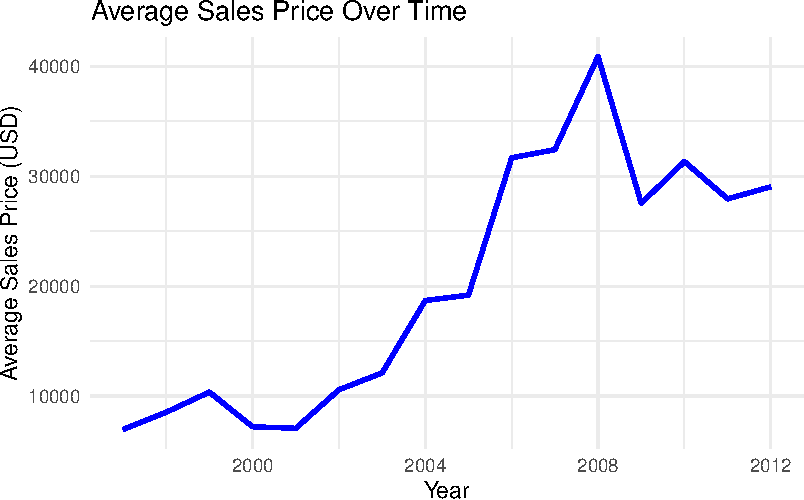
\includegraphics{506-HW-5_files/figure-pdf/unnamed-chunk-7-1.pdf}

\textbf{Redefining Column Data}

\begin{Shaded}
\begin{Highlighting}[]
\NormalTok{art\_sales }\OtherTok{\textless{}{-}}\NormalTok{ art\_sales }\SpecialCharTok{\%\textgreater{}\%}
  \FunctionTok{mutate}\NormalTok{(}\AttributeTok{genre =} \FunctionTok{case\_when}\NormalTok{(}
\NormalTok{    Genre\_\_\_Photography }\SpecialCharTok{==} \DecValTok{1} \SpecialCharTok{\textasciitilde{}} \StringTok{"Photography"}\NormalTok{,}
\NormalTok{    Genre\_\_\_Print }\SpecialCharTok{==} \DecValTok{1} \SpecialCharTok{\textasciitilde{}} \StringTok{"Print"}\NormalTok{,}
\NormalTok{    Genre\_\_\_Sculpture }\SpecialCharTok{==} \DecValTok{1} \SpecialCharTok{\textasciitilde{}} \StringTok{"Sculpture"}\NormalTok{,}
\NormalTok{    Genre\_\_\_Painting }\SpecialCharTok{==} \DecValTok{1} \SpecialCharTok{\textasciitilde{}} \StringTok{"Painting"}\NormalTok{,}
\NormalTok{    Genre\_\_\_Others }\SpecialCharTok{==} \DecValTok{1} \SpecialCharTok{\textasciitilde{}} \StringTok{"Others"}\NormalTok{,}
    \ConstantTok{TRUE} \SpecialCharTok{\textasciitilde{}} \ConstantTok{NA\_character\_}  
\NormalTok{  ))}
\FunctionTok{print}\NormalTok{(}\FunctionTok{head}\NormalTok{(art\_sales[[}\DecValTok{113}\NormalTok{]],}\DecValTok{10}\NormalTok{)) }\CommentTok{\# checking if transformation }
\end{Highlighting}
\end{Shaded}

\begin{verbatim}
 [1] "Painting"    "Sculpture"   "Sculpture"   "Painting"    "Photography"
 [6] "Painting"    "Painting"    "Painting"    "Painting"    "Sculpture"  
\end{verbatim}

\begin{Shaded}
\begin{Highlighting}[]
                                \CommentTok{\# was successful }
\end{Highlighting}
\end{Shaded}

\textbf{Fluctuation in the selling price of each genre over time}

\begin{Shaded}
\begin{Highlighting}[]
\NormalTok{genre\_distribution }\OtherTok{\textless{}{-}}\NormalTok{ art\_sales }\SpecialCharTok{\%\textgreater{}\%}
  \FunctionTok{group\_by}\NormalTok{(year,genre) }\SpecialCharTok{\%\textgreater{}\%}
  \FunctionTok{summarise}\NormalTok{(}\AttributeTok{num\_sales =} \FunctionTok{n}\NormalTok{()) }\SpecialCharTok{\%\textgreater{}\%}
  \FunctionTok{ggplot}\NormalTok{(}\FunctionTok{aes}\NormalTok{(}\AttributeTok{x =}\NormalTok{ year, }\AttributeTok{y =}\NormalTok{ num\_sales, }\AttributeTok{fill =}\NormalTok{ genre)) }\SpecialCharTok{+}
  \FunctionTok{geom\_bar}\NormalTok{(}\AttributeTok{stat =} \StringTok{"identity"}\NormalTok{, }\AttributeTok{position =} \StringTok{"stack"}\NormalTok{) }\SpecialCharTok{+}
  \FunctionTok{labs}\NormalTok{(}\AttributeTok{title =} \StringTok{"Distribution of Genres Over Time"}\NormalTok{, }\AttributeTok{x =} \StringTok{"Year"}\NormalTok{, }\AttributeTok{y =} \StringTok{"Number of Sales"}\NormalTok{) }\SpecialCharTok{+}
  \FunctionTok{theme\_minimal}\NormalTok{() }\SpecialCharTok{+}
  \FunctionTok{theme}\NormalTok{(}\AttributeTok{legend.position =} \StringTok{"bottom"}\NormalTok{)}
\end{Highlighting}
\end{Shaded}

\begin{verbatim}
`summarise()` has grouped output by 'year'. You can override using the
`.groups` argument.
\end{verbatim}

\begin{Shaded}
\begin{Highlighting}[]
\DocumentationTok{\#\# Display plot}
\NormalTok{genre\_distribution}
\end{Highlighting}
\end{Shaded}

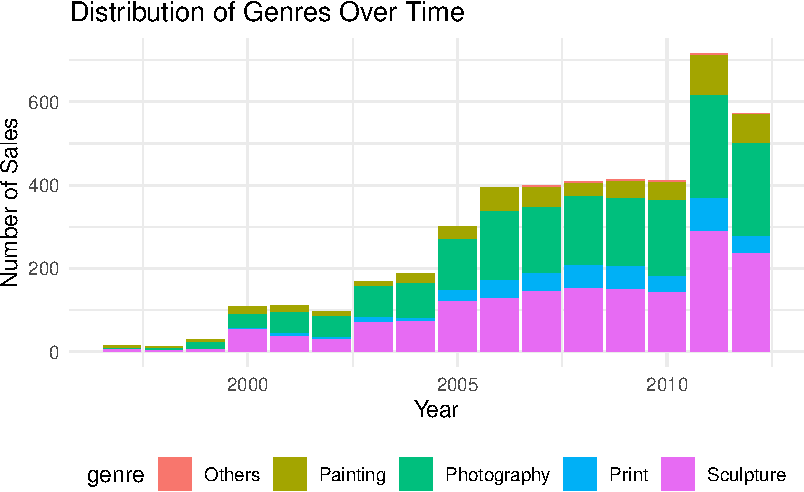
\includegraphics{506-HW-5_files/figure-pdf/unnamed-chunk-9-1.pdf}

\subsubsection{\texorpdfstring{2 - Interactive plot with
\texttt{plotly()}}{2 - Interactive plot with plotly()}}\label{interactive-plot-with-plotly}

\begin{Shaded}
\begin{Highlighting}[]
\FunctionTok{library}\NormalTok{(htmlwidgets)}
  
\NormalTok{plot }\OtherTok{\textless{}{-}} \FunctionTok{plot\_ly}\NormalTok{(art\_sales, }\AttributeTok{x =} \SpecialCharTok{\textasciitilde{}}\NormalTok{year, }\AttributeTok{y =} \SpecialCharTok{\textasciitilde{}}\NormalTok{price\_usd, }\AttributeTok{color =} \SpecialCharTok{\textasciitilde{}}\NormalTok{genre, }\AttributeTok{type =} \StringTok{\textquotesingle{}scatter\textquotesingle{}}\NormalTok{, }\AttributeTok{mode =} \StringTok{\textquotesingle{}lines+markers\textquotesingle{}}\NormalTok{) }\SpecialCharTok{\%\textgreater{}\%}
  \FunctionTok{layout}\NormalTok{(}
    \AttributeTok{title =} \StringTok{"Change in Sales Price Over Time by Genre"}\NormalTok{,}
    \AttributeTok{xaxis =} \FunctionTok{list}\NormalTok{(}\AttributeTok{title =} \StringTok{"Year"}\NormalTok{),}
    \AttributeTok{yaxis =} \FunctionTok{list}\NormalTok{(}\AttributeTok{title =} \StringTok{"Sales Price (USD)"}\NormalTok{),}
    \AttributeTok{legend =} \FunctionTok{list}\NormalTok{(}\AttributeTok{title =} \FunctionTok{list}\NormalTok{(}\AttributeTok{text =} \StringTok{"Genre"}\NormalTok{))}
\NormalTok{  )}

\CommentTok{\# Save the plot as an HTML file}
\FunctionTok{saveWidget}\NormalTok{(plot, }\StringTok{"interactive\_plot.html"}\NormalTok{)}
\end{Highlighting}
\end{Shaded}

\textbf{You can view the interactive plot by clicking
\href{./interactive_plot.html}{here}.}

Or, paste this network-link into the web-browser
\url{file:///C:/Users/vasud/OneDrive/Desktop/U-M\%20-\%20ALL/STATS\%20506/HW-5/interactive_plot.html}

\hfill\break

\begin{center}\rule{0.5\linewidth}{0.5pt}\end{center}

\subsection{Problem - 3}\label{problem---3}

\subsubsection{Solution to HW-4 Problem-1 using
data.table}\label{solution-to-hw-4-problem-1-using-data.table}

\begin{Shaded}
\begin{Highlighting}[]
\FunctionTok{library}\NormalTok{(data.table)}
\end{Highlighting}
\end{Shaded}

\begin{verbatim}
Warning: package 'data.table' was built under R version 4.4.2
\end{verbatim}

\begin{verbatim}

Attaching package: 'data.table'
\end{verbatim}

\begin{verbatim}
The following objects are masked from 'package:dplyr':

    between, first, last
\end{verbatim}

\begin{Shaded}
\begin{Highlighting}[]
\FunctionTok{library}\NormalTok{(nycflights13)}
\FunctionTok{library}\NormalTok{(kableExtra)}
\end{Highlighting}
\end{Shaded}

\begin{verbatim}

Attaching package: 'kableExtra'
\end{verbatim}

\begin{verbatim}
The following object is masked from 'package:dplyr':

    group_rows
\end{verbatim}

\begin{Shaded}
\begin{Highlighting}[]
\FunctionTok{library}\NormalTok{(knitr)}
\end{Highlighting}
\end{Shaded}

\begin{verbatim}
Warning: package 'knitr' was built under R version 4.4.2
\end{verbatim}

\begin{Shaded}
\begin{Highlighting}[]
\CommentTok{\# Convert relevant datasets to data.table}
\NormalTok{flights\_dt }\OtherTok{\textless{}{-}} \FunctionTok{as.data.table}\NormalTok{(flights)}
\NormalTok{airports\_dt }\OtherTok{\textless{}{-}} \FunctionTok{as.data.table}\NormalTok{(airports)}
\NormalTok{planes\_dt }\OtherTok{\textless{}{-}} \FunctionTok{as.data.table}\NormalTok{(planes)}

\CommentTok{\# Departure delay summary}
\NormalTok{departure\_delay\_summary }\OtherTok{\textless{}{-}}\NormalTok{ flights\_dt[}
  \SpecialCharTok{!}\FunctionTok{is.na}\NormalTok{(dep\_delay), }\CommentTok{\# Exclude rows with NA dep\_delay}
\NormalTok{  .(}
    \StringTok{\textasciigrave{}}\AttributeTok{Mean Delay}\StringTok{\textasciigrave{}} \OtherTok{=} \FunctionTok{mean}\NormalTok{(dep\_delay, }\AttributeTok{na.rm =} \ConstantTok{TRUE}\NormalTok{),}
    \StringTok{\textasciigrave{}}\AttributeTok{Median Delay}\StringTok{\textasciigrave{}} \OtherTok{=} \FunctionTok{median}\NormalTok{(dep\_delay, }\AttributeTok{na.rm =} \ConstantTok{TRUE}\NormalTok{),}
    \AttributeTok{Flights =}\NormalTok{ .N}
\NormalTok{  ), by }\OtherTok{=}\NormalTok{ dest}
\NormalTok{][}
\NormalTok{  Flights }\SpecialCharTok{\textgreater{}=} \DecValTok{10}
\NormalTok{][}
  \FunctionTok{order}\NormalTok{(}\SpecialCharTok{{-}}\StringTok{\textasciigrave{}}\AttributeTok{Mean Delay}\StringTok{\textasciigrave{}}\NormalTok{)}
\NormalTok{][}
\NormalTok{  airports\_dt, on }\OtherTok{=}\NormalTok{ .(}\AttributeTok{dest =}\NormalTok{ faa), nomatch }\OtherTok{=} \DecValTok{0}
\NormalTok{][}
\NormalTok{  , .(name, }\StringTok{\textasciigrave{}}\AttributeTok{Mean Delay}\StringTok{\textasciigrave{}}\NormalTok{, }\StringTok{\textasciigrave{}}\AttributeTok{Median Delay}\StringTok{\textasciigrave{}}\NormalTok{, Flights) }\CommentTok{\# Use the column directly after the join}
\NormalTok{]}

\ControlFlowTok{if}\NormalTok{ (}\FunctionTok{nrow}\NormalTok{(departure\_delay\_summary) }\SpecialCharTok{==} \DecValTok{0}\NormalTok{) \{}
\NormalTok{  departure\_delay\_summary }\OtherTok{\textless{}{-}} \FunctionTok{data.table}\NormalTok{(}\AttributeTok{name =} \ConstantTok{NA}\NormalTok{, }\StringTok{\textasciigrave{}}\AttributeTok{Mean Delay}\StringTok{\textasciigrave{}} \OtherTok{=} \ConstantTok{NA}\NormalTok{, }\StringTok{\textasciigrave{}}\AttributeTok{Median Delay}\StringTok{\textasciigrave{}} \OtherTok{=} \ConstantTok{NA}\NormalTok{, }\AttributeTok{Flights =} \ConstantTok{NA}\NormalTok{)}
\NormalTok{\}}

\FunctionTok{kable}\NormalTok{(departure\_delay\_summary, }\AttributeTok{caption =} \StringTok{"Departure Delays"}\NormalTok{, }\AttributeTok{digits =} \DecValTok{1}\NormalTok{, }\AttributeTok{align =} \StringTok{\textquotesingle{}c\textquotesingle{}}\NormalTok{)}
\end{Highlighting}
\end{Shaded}

\begin{longtable}[]{@{}
  >{\centering\arraybackslash}p{(\columnwidth - 6\tabcolsep) * \real{0.5205}}
  >{\centering\arraybackslash}p{(\columnwidth - 6\tabcolsep) * \real{0.1644}}
  >{\centering\arraybackslash}p{(\columnwidth - 6\tabcolsep) * \real{0.1918}}
  >{\centering\arraybackslash}p{(\columnwidth - 6\tabcolsep) * \real{0.1233}}@{}}
\caption{Departure Delays}\tabularnewline
\toprule\noalign{}
\begin{minipage}[b]{\linewidth}\centering
name
\end{minipage} & \begin{minipage}[b]{\linewidth}\centering
Mean Delay
\end{minipage} & \begin{minipage}[b]{\linewidth}\centering
Median Delay
\end{minipage} & \begin{minipage}[b]{\linewidth}\centering
Flights
\end{minipage} \\
\midrule\noalign{}
\endfirsthead
\toprule\noalign{}
\begin{minipage}[b]{\linewidth}\centering
name
\end{minipage} & \begin{minipage}[b]{\linewidth}\centering
Mean Delay
\end{minipage} & \begin{minipage}[b]{\linewidth}\centering
Median Delay
\end{minipage} & \begin{minipage}[b]{\linewidth}\centering
Flights
\end{minipage} \\
\midrule\noalign{}
\endhead
\bottomrule\noalign{}
\endlastfoot
Albuquerque International Sunport & 13.7 & 0.0 & 254 \\
Nantucket Mem & 6.5 & -3.0 & 265 \\
Albany Intl & 23.6 & 1.0 & 419 \\
Hartsfield Jackson Atlanta Intl & 12.5 & -2.0 & 16898 \\
Austin Bergstrom Intl & 13.0 & -1.0 & 2418 \\
Asheville Regional Airport & 8.2 & -3.0 & 263 \\
Bradley Intl & 17.7 & -1.0 & 412 \\
Bangor Intl & 19.5 & -2.0 & 360 \\
Birmingham Intl & 29.7 & 1.0 & 272 \\
Nashville Intl & 16.0 & -1.0 & 6104 \\
General Edward Lawrence Logan Intl & 8.7 & -3.0 & 15049 \\
Burlington Intl & 13.6 & -2.0 & 2513 \\
Buffalo Niagara Intl & 13.4 & -2.0 & 4576 \\
Bob Hope & 13.5 & -1.0 & 370 \\
Baltimore Washington Intl & 16.4 & -2.0 & 1696 \\
Gallatin Field & 11.5 & 0.0 & 35 \\
Columbia Metropolitan & 35.6 & 14.0 & 107 \\
Akron Canton Regional Airport & 20.8 & 0.0 & 843 \\
Charlottesville-Albemarle & 21.4 & -2.5 & 46 \\
Charleston Afb Intl & 14.7 & -2.0 & 2775 \\
Cleveland Hopkins Intl & 13.4 & -2.0 & 4408 \\
Charlotte Douglas Intl & 9.2 & -3.0 & 13698 \\
Port Columbus Intl & 12.2 & -3.0 & 3338 \\
Yeager & 17.0 & -4.0 & 137 \\
Cincinnati Northern Kentucky Intl & 19.5 & -2.0 & 3740 \\
James M Cox Dayton Intl & 17.5 & -2.0 & 1402 \\
Ronald Reagan Washington Natl & 10.3 & -3.0 & 9157 \\
Denver Intl & 15.2 & 1.0 & 7201 \\
Dallas Fort Worth Intl & 8.7 & -3.0 & 8463 \\
Des Moines Intl & 26.2 & -1.0 & 528 \\
Detroit Metro Wayne Co & 11.8 & -3.0 & 9060 \\
Eagle Co Rgnl & 15.5 & -1.0 & 208 \\
Key West Intl & 3.6 & 0.0 & 17 \\
Fort Lauderdale Hollywood Intl & 12.7 & -1.0 & 11934 \\
Gerald R Ford Intl & 19.5 & -1.0 & 735 \\
Piedmont Triad & 19.4 & -1.0 & 1500 \\
Greenville-Spartanburg International & 19.3 & -1.0 & 794 \\
Yampa Valley & 12.3 & 6.5 & 14 \\
Honolulu Intl & 9.3 & -1.0 & 705 \\
William P Hobby & 14.3 & 0.0 & 2090 \\
Washington Dulles Intl & 17.0 & -2.0 & 5391 \\
George Bush Intercontinental & 10.8 & 0.0 & 7103 \\
Wilmington Intl & 19.4 & -3.0 & 108 \\
Indianapolis Intl & 14.0 & -2.0 & 1991 \\
Jackson Hole Airport & 26.5 & 13.5 & 22 \\
Jacksonville Intl & 16.5 & -1.0 & 2634 \\
Mc Carran Intl & 9.4 & -1.0 & 5962 \\
Los Angeles Intl & 9.4 & -1.0 & 16076 \\
Long Beach & 11.2 & -1.0 & 664 \\
Kansas City Intl & 20.3 & -1.0 & 1896 \\
Orlando Intl & 11.3 & -1.0 & 13982 \\
Chicago Midway Intl & 18.6 & 2.0 & 4044 \\
Memphis Intl & 15.7 & -1.0 & 1694 \\
Manchester Regional Airport & 21.0 & 0.0 & 932 \\
Miami Intl & 8.9 & -2.0 & 11633 \\
General Mitchell Intl & 18.8 & 0.0 & 2718 \\
Dane Co Rgnl Truax Fld & 23.6 & -1.0 & 562 \\
Minneapolis St Paul Intl & 13.3 & -2.0 & 6958 \\
Louis Armstrong New Orleans Intl & 14.2 & -2.0 & 3724 \\
Montrose Regional Airport & 17.6 & 3.0 & 14 \\
Martha\textbackslash's Vineyard & 7.1 & -2.0 & 213 \\
Myrtle Beach Intl & 15.8 & -1.0 & 58 \\
Metropolitan Oakland Intl & 13.3 & 0.0 & 311 \\
Will Rogers World & 30.6 & 10.0 & 327 \\
Eppley Afld & 20.2 & -1.0 & 822 \\
Chicago Ohare Intl & 13.6 & -2.0 & 16642 \\
Norfolk Intl & 17.6 & -2.0 & 1440 \\
Palm Beach Intl & 13.0 & 0.0 & 6495 \\
Portland Intl & 16.3 & 1.0 & 1348 \\
Philadelphia Intl & 12.0 & -3.0 & 1549 \\
Phoenix Sky Harbor Intl & 10.4 & -1.0 & 4611 \\
Pittsburgh Intl & 13.7 & -2.0 & 2759 \\
Palm Springs Intl & -2.9 & -4.0 & 18 \\
Theodore Francis Green State & 21.8 & 0.0 & 358 \\
Portland Intl Jetport & 16.5 & -2.0 & 2295 \\
Raleigh Durham Intl & 12.4 & -2.0 & 7796 \\
Richmond Intl & 23.6 & -1.0 & 2349 \\
Greater Rochester Intl & 16.2 & -2.0 & 2362 \\
Southwest Florida Intl & 8.3 & -2.0 & 3509 \\
San Diego Intl & 11.1 & 0.0 & 2724 \\
San Antonio Intl & 20.7 & 1.0 & 678 \\
Savannah Hilton Head Intl & 18.3 & -1.0 & 753 \\
South Bend Rgnl & 21.1 & 14.0 & 10 \\
Louisville International Airport & 16.4 & -2.0 & 1117 \\
Seattle Tacoma Intl & 10.7 & -1.0 & 3904 \\
San Francisco Intl & 12.9 & 0.0 & 13230 \\
Norman Y Mineta San Jose Intl & 10.1 & -1.0 & 328 \\
Salt Lake City Intl & 9.0 & -1.0 & 2458 \\
Sacramento Intl & 18.7 & 2.0 & 282 \\
John Wayne Arpt Orange Co & 7.8 & -1.0 & 819 \\
Sarasota Bradenton Intl & 7.3 & -3.0 & 1203 \\
Lambert St Louis Intl & 16.0 & -1.0 & 4168 \\
Syracuse Hancock Intl & 14.4 & -2.0 & 1711 \\
Tampa Intl & 12.1 & -1.0 & 7407 \\
Tulsa Intl & 34.9 & 8.0 & 299 \\
Cherry Capital Airport & 22.1 & -3.0 & 96 \\
Mc Ghee Tyson & 28.5 & 0.0 & 579 \\
NW Arkansas Regional & 6.5 & -5.0 & 1011 \\
\end{longtable}

\begin{Shaded}
\begin{Highlighting}[]
\CommentTok{\# Arrival delay summary}
\NormalTok{arrival\_delay\_summary }\OtherTok{\textless{}{-}}\NormalTok{ flights\_dt[}
  \SpecialCharTok{!}\FunctionTok{is.na}\NormalTok{(arr\_delay), }\CommentTok{\# Exclude rows with NA arr\_delay}
\NormalTok{  .(}
    \AttributeTok{mean\_arr\_delay =} \FunctionTok{mean}\NormalTok{(arr\_delay, }\AttributeTok{na.rm =} \ConstantTok{TRUE}\NormalTok{),}
    \AttributeTok{median\_arr\_delay =} \FunctionTok{median}\NormalTok{(arr\_delay, }\AttributeTok{na.rm =} \ConstantTok{TRUE}\NormalTok{),}
    \AttributeTok{num\_flights =}\NormalTok{ .N}
\NormalTok{  ), by }\OtherTok{=}\NormalTok{ dest}
\NormalTok{][}
\NormalTok{  num\_flights }\SpecialCharTok{\textgreater{}=} \DecValTok{10}
\NormalTok{][}
  \FunctionTok{order}\NormalTok{(}\SpecialCharTok{{-}}\NormalTok{mean\_arr\_delay)}
\NormalTok{][}
\NormalTok{  airports\_dt, on }\OtherTok{=}\NormalTok{ .(}\AttributeTok{dest =}\NormalTok{ faa), nomatch }\OtherTok{=} \DecValTok{0}
\NormalTok{][}
\NormalTok{  , .(name, mean\_arr\_delay, median\_arr\_delay, num\_flights) }\CommentTok{\# Use the column directly after the join}
\NormalTok{]}

\ControlFlowTok{if}\NormalTok{ (}\FunctionTok{nrow}\NormalTok{(arrival\_delay\_summary) }\SpecialCharTok{==} \DecValTok{0}\NormalTok{) \{}
\NormalTok{  arrival\_delay\_summary }\OtherTok{\textless{}{-}} \FunctionTok{data.table}\NormalTok{(}\AttributeTok{name =} \ConstantTok{NA}\NormalTok{, }\AttributeTok{mean\_arr\_delay =} \ConstantTok{NA}\NormalTok{, }\AttributeTok{median\_arr\_delay =} \ConstantTok{NA}\NormalTok{, }\AttributeTok{num\_flights =} \ConstantTok{NA}\NormalTok{)}
\NormalTok{\}}

\FunctionTok{kable}\NormalTok{(arrival\_delay\_summary, }\AttributeTok{align =} \StringTok{\textquotesingle{}c\textquotesingle{}}\NormalTok{)}
\end{Highlighting}
\end{Shaded}

\begin{longtable}[]{@{}
  >{\centering\arraybackslash}p{(\columnwidth - 6\tabcolsep) * \real{0.4471}}
  >{\centering\arraybackslash}p{(\columnwidth - 6\tabcolsep) * \real{0.1882}}
  >{\centering\arraybackslash}p{(\columnwidth - 6\tabcolsep) * \real{0.2118}}
  >{\centering\arraybackslash}p{(\columnwidth - 6\tabcolsep) * \real{0.1529}}@{}}
\toprule\noalign{}
\begin{minipage}[b]{\linewidth}\centering
name
\end{minipage} & \begin{minipage}[b]{\linewidth}\centering
mean\_arr\_delay
\end{minipage} & \begin{minipage}[b]{\linewidth}\centering
median\_arr\_delay
\end{minipage} & \begin{minipage}[b]{\linewidth}\centering
num\_flights
\end{minipage} \\
\midrule\noalign{}
\endhead
\bottomrule\noalign{}
\endlastfoot
Albuquerque International Sunport & 4.3818898 & -5.5 & 254 \\
Nantucket Mem & 4.8522727 & -3.0 & 264 \\
Albany Intl & 14.3971292 & -4.0 & 418 \\
Hartsfield Jackson Atlanta Intl & 11.3001128 & -1.0 & 16837 \\
Austin Bergstrom Intl & 6.0199088 & -5.0 & 2411 \\
Asheville Regional Airport & 8.0038314 & -1.0 & 261 \\
Bradley Intl & 7.0485437 & -10.0 & 412 \\
Bangor Intl & 8.0279330 & -9.0 & 358 \\
Birmingham Intl & 16.8773234 & -2.0 & 269 \\
Nashville Intl & 11.8124589 & -2.0 & 6084 \\
General Edward Lawrence Logan Intl & 2.9143922 & -9.0 & 15022 \\
Burlington Intl & 8.9509960 & -4.0 & 2510 \\
Buffalo Niagara Intl & 8.9459519 & -5.0 & 4570 \\
Bob Hope & 8.1756757 & -3.0 & 370 \\
Baltimore Washington Intl & 10.7267338 & -5.0 & 1687 \\
Gallatin Field & 7.6000000 & -2.0 & 35 \\
Columbia Metropolitan & 41.7641509 & 28.0 & 106 \\
Akron Canton Regional Airport & 19.6983373 & 3.0 & 842 \\
Charlottesville-Albemarle & 9.5000000 & -5.0 & 46 \\
Charleston Afb Intl & 10.5929685 & -4.0 & 2759 \\
Cleveland Hopkins Intl & 9.1816113 & -5.0 & 4394 \\
Charlotte Douglas Intl & 7.3603189 & -3.0 & 13674 \\
Port Columbus Intl & 10.6013229 & -3.0 & 3326 \\
Yeager & 14.6716418 & -1.5 & 134 \\
Cincinnati Northern Kentucky Intl & 15.3645638 & -3.0 & 3725 \\
James M Cox Dayton Intl & 12.6804861 & -3.0 & 1399 \\
Ronald Reagan Washington Natl & 9.0669520 & -2.0 & 9111 \\
Denver Intl & 8.6065002 & -2.0 & 7169 \\
Dallas Fort Worth Intl & 0.3221268 & -9.0 & 8388 \\
Des Moines Intl & 19.0057361 & 0.0 & 523 \\
Detroit Metro Wayne Co & 5.4299635 & -7.0 & 9031 \\
Eagle Co Rgnl & 6.3043478 & -4.0 & 207 \\
Key West Intl & 6.3529412 & 7.0 & 17 \\
Fort Lauderdale Hollywood Intl & 8.0821215 & -3.0 & 11897 \\
Gerald R Ford Intl & 18.1895604 & 1.0 & 728 \\
Piedmont Triad & 14.1126005 & -2.0 & 1492 \\
Greenville-Spartanburg International & 15.9354430 & -0.5 & 790 \\
Yampa Valley & 2.1428571 & 2.0 & 14 \\
Honolulu Intl & -1.3651926 & -7.0 & 701 \\
William P Hobby & 7.1761882 & -4.0 & 2083 \\
Washington Dulles Intl & 13.8642021 & -3.0 & 5383 \\
George Bush Intercontinental & 4.2407904 & -5.0 & 7085 \\
Wilmington Intl & 4.6355140 & -7.0 & 107 \\
Indianapolis Intl & 9.9404341 & -3.0 & 1981 \\
Jackson Hole Airport & 28.0952381 & 15.0 & 21 \\
Jacksonville Intl & 11.8448342 & -2.0 & 2623 \\
Mc Carran Intl & 0.2577285 & -8.0 & 5952 \\
Los Angeles Intl & 0.5471109 & -7.0 & 16026 \\
Long Beach & -0.0620272 & -10.0 & 661 \\
Kansas City Intl & 14.5140584 & 0.0 & 1885 \\
Orlando Intl & 5.4546431 & -5.0 & 13967 \\
Chicago Midway Intl & 12.3642236 & -1.0 & 4025 \\
Memphis Intl & 10.6453144 & -2.5 & 1686 \\
Manchester Regional Airport & 14.7875536 & -3.0 & 932 \\
Miami Intl & 0.2990598 & -9.0 & 11593 \\
General Mitchell Intl & 14.1672204 & 0.0 & 2709 \\
Dane Co Rgnl Truax Fld & 20.1960432 & 1.0 & 556 \\
Minneapolis St Paul Intl & 7.2701689 & -5.0 & 6929 \\
Louis Armstrong New Orleans Intl & 6.4901750 & -6.0 & 3715 \\
Montrose Regional Airport & 1.7857143 & -10.5 & 14 \\
Martha\textbackslash's Vineyard & -0.2857143 & -11.0 & 210 \\
Myrtle Beach Intl & 4.6034483 & -13.0 & 58 \\
Metropolitan Oakland Intl & 3.0776699 & -9.0 & 309 \\
Will Rogers World & 30.6190476 & 16.0 & 315 \\
Eppley Afld & 14.6988984 & -2.0 & 817 \\
Chicago Ohare Intl & 5.8766148 & -8.0 & 16566 \\
Norfolk Intl & 10.9490934 & -4.0 & 1434 \\
Palm Beach Intl & 8.5629721 & -3.0 & 6487 \\
Portland Intl & 5.1415797 & -5.0 & 1342 \\
Philadelphia Intl & 10.1271901 & -3.0 & 1541 \\
Phoenix Sky Harbor Intl & 2.0970473 & -6.0 & 4606 \\
Pittsburgh Intl & 7.6809905 & -5.0 & 2746 \\
Palm Springs Intl & -12.7222222 & -13.5 & 18 \\
Theodore Francis Green State & 16.2346369 & 1.0 & 358 \\
Portland Intl Jetport & 11.6604021 & -4.0 & 2288 \\
Raleigh Durham Intl & 10.0523810 & -3.0 & 7770 \\
Richmond Intl & 20.1112532 & 1.0 & 2346 \\
Greater Rochester Intl & 11.5606446 & -5.0 & 2358 \\
Southwest Florida Intl & 3.2381496 & -5.0 & 3502 \\
San Diego Intl & 3.1391657 & -5.0 & 2709 \\
San Antonio Intl & 6.9453718 & -9.0 & 659 \\
Savannah Hilton Head Intl & 15.1295060 & -1.0 & 749 \\
South Bend Rgnl & 6.5000000 & -3.5 & 10 \\
Louisville International Airport & 12.6693841 & -2.0 & 1104 \\
Seattle Tacoma Intl & -1.0990991 & -11.0 & 3885 \\
San Francisco Intl & 2.6728915 & -8.0 & 13173 \\
Norman Y Mineta San Jose Intl & 3.4481707 & -7.0 & 328 \\
Salt Lake City Intl & 0.1762546 & -8.0 & 2451 \\
Sacramento Intl & 12.1099291 & 4.0 & 282 \\
John Wayne Arpt Orange Co & -7.8682266 & -11.0 & 812 \\
Sarasota Bradenton Intl & 3.0824313 & -5.0 & 1201 \\
Lambert St Louis Intl & 11.0784645 & -3.0 & 4142 \\
Syracuse Hancock Intl & 8.9039250 & -5.0 & 1707 \\
Tampa Intl & 7.4085250 & -4.0 & 7390 \\
Tulsa Intl & 33.6598639 & 14.0 & 294 \\
Cherry Capital Airport & 12.9684211 & -10.0 & 95 \\
Mc Ghee Tyson & 24.0692042 & 2.0 & 578 \\
NW Arkansas Regional & 7.4657258 & -2.0 & 992 \\
\end{longtable}

\begin{Shaded}
\begin{Highlighting}[]
\CommentTok{\# Calculate speed}
\NormalTok{flights\_dt[, speed\_mph }\SpecialCharTok{:}\ErrorTok{=}\NormalTok{ distance }\SpecialCharTok{/}\NormalTok{ (air\_time }\SpecialCharTok{/} \DecValTok{60}\NormalTok{)]}
\NormalTok{flights\_dt }\OtherTok{\textless{}{-}}\NormalTok{ flights\_dt[}\SpecialCharTok{!}\FunctionTok{is.na}\NormalTok{(speed\_mph)] }\CommentTok{\# Exclude rows with NA speeds}

\CommentTok{\# Find the aircraft with the fastest average speed}
\NormalTok{fastest\_aircraft }\OtherTok{\textless{}{-}}\NormalTok{ flights\_dt[}
\NormalTok{  , .(}
    \AttributeTok{avg\_speed =} \FunctionTok{mean}\NormalTok{(speed\_mph, }\AttributeTok{na.rm =} \ConstantTok{TRUE}\NormalTok{),}
    \AttributeTok{num\_flights =}\NormalTok{ .N}
\NormalTok{  ), by }\OtherTok{=}\NormalTok{ tailnum}
\NormalTok{][}
  \FunctionTok{order}\NormalTok{(}\SpecialCharTok{{-}}\NormalTok{avg\_speed)}
\NormalTok{][}
  \DecValTok{1}
\NormalTok{]}

\ControlFlowTok{if}\NormalTok{ (}\FunctionTok{nrow}\NormalTok{(fastest\_aircraft) }\SpecialCharTok{==} \DecValTok{0}\NormalTok{) \{}
\NormalTok{  fastest\_model }\OtherTok{\textless{}{-}} \FunctionTok{data.table}\NormalTok{(}\AttributeTok{model =} \ConstantTok{NA}\NormalTok{, }\AttributeTok{avg\_speed =} \ConstantTok{NA}\NormalTok{, }\AttributeTok{num\_flights =} \ConstantTok{NA}\NormalTok{)}
\NormalTok{\} }\ControlFlowTok{else}\NormalTok{ \{}
  \CommentTok{\# Join with planes to get the model}
\NormalTok{  fastest\_model }\OtherTok{\textless{}{-}}\NormalTok{ fastest\_aircraft[}
\NormalTok{    planes\_dt, on }\OtherTok{=} \StringTok{"tailnum"}\NormalTok{, nomatch }\OtherTok{=} \DecValTok{0}
\NormalTok{  ][}
\NormalTok{    , .(model, avg\_speed, num\_flights)}
\NormalTok{  ]}
\NormalTok{\}}

\CommentTok{\# Display the fastest model}
\NormalTok{fastest\_model}
\end{Highlighting}
\end{Shaded}

\begin{verbatim}
     model avg_speed num_flights
    <char>     <num>       <int>
1: 777-222  500.8163           1
\end{verbatim}

\ul{\textbf{The computed results can be compared back to HW-4. They are
precisely the same.}}




\end{document}
